% !TeX root = RJwrapper.tex
\title{rfPermute: Estimation of Predictor Importance Significance in Random
Forest Models}
\author{by Frederick I. Archer}

\maketitle

\abstract{%
``One of the strengths of the ensemble machine learning algorithm,
Random Forest, is its ability to estimate the relative importance of
predictors within classification and regression models. However, there
is no method for identifying which predictors are significantly more
important than what would be expected by random chance. I present the
\emph{rfPermute} package which is a wrapper for the commonly used
\emph{randomForest} package that produces permutation based estimates of
predictor importance significance. The package also includes utility
functions for summarizing and visualizing Random Forest model results.''
}

\subsection{Introduction}\label{introduction}

Introductory section which may include references in parentheses
\citep{R}, or cite a reference such as \citet{R} in the text.

\subsection{Introduction}\label{introduction-1}

Since its inception, the ensemble machine learning algorithm, Random
Forest (Breiman 2001), has been rapidly gaining popularity as a powerful
tool for classification and uncovering patterns in complex data sets. It
has been used a wide variety of fields (Cutler et al. 2007, Winham et
al. 2012, Touw et al. 2012), and has proven to be robust in performance
tests against other commonly used modelling algorithms (Berk 2006).

The most commonly used implementation of Random Forest is the
\emph{randomForest} package in R (Liaw and Weiner 2002). This package
allows easy specification of both classification and regression models
and provides several useful functions for summarizing their results. One
of the metrics that many users of Random Forest are interested in
examining are the measures of variable or predictor importance. The
importance of a predictor is estimated by measuring the decrease in
prediction accuracy when that predictor is permuted in each tree in the
forest. These values are often used to identify and rank those
predictors that are most related to the response and critical for
classification. More detail about how the various importance metrics are
computed can be found in Liaw and Weiner (2002) and Breiman (2002).

However, \emph{randomForest} only produces raw measures of predictor
importance and it is up to the user to identify cutoff values above
which predictors would be considered to have a significant impact on
model predictions. In order to address this, I have implemented a
permutation test in \emph{rfPermute} which generates a null distribution
of importance scores for each predictor against which the observed
importance scores are compared. This null distribution is created by
randomly permuting the response variable (class assignments in a
classification model, or independent continuous response in a regression
model) among cases, running the same Random Forest model on the permuted
data, and storing the resulting importance scores.

Under this procedure, a predictor that is not adding any significant
information to the model will have an observed importance score that is
similar to those generated by a random shuffling of the response, while
a significant predictor will have an importance score much larger than
the null. Significance p-values are then calculated as the fraction of
replicates in the null distribution that are greater than or equal to
the observed value. \emph{rfPermute} provides both the p-values and the
null distribution which the user can use for variable selection and
further exploration.

\subsection{Execution}\label{execution}

\emph{rfPermute} provides a wrapper for the \emph{randomForest} function
that accepts all of its arguments, plus two additional ones:
\emph{nrep}, which is an integer specifying the number of permutation
replicates to run, and \emph{num.cores}, which is an integer specifying
the number of CPU cores to distribute the permutations over on a
multi-core system. If \emph{nrep} is set to 0, then the return value is
a list with the same elements as the equivalent call to
\emph{randomForest}. With one or more permutation replicates specified,
the returned list contains two elements: \emph{null.dist}, which is a
list containing arrays of the null distributions for unscaled and scaled
importance measures, and \emph{pval}, which is an array containing the
permutation p-values for unscaled and scaled importance measures.

As an example, we use a data set of metabolite profiles measured to
create a classifier for four clades of the endosymbiont dinoflagellate
\emph{Symbiodinium} as published in Klueter et al (2015). Significance
is measured with 1000 permutations. Because each \emph{Symbiodinium}
type is represented by 16 cases in this data set, we create a model
where 8 cases from each type are used in each tree and sampling is done
without replacement. \emph{rfPermute} automatically sets
\texttt{importance\ =\ TRUE} to force \texttt{randomForest} to calculate
and return the matrix of importance scores, so we don't need to set
that. However, we will be using the proximity matrix later, so we must
specify \texttt{proximity\ =\ TRUE}.

\begin{Schunk}
\begin{Sinput}
# Load the package
library(rfPermute)
\end{Sinput}
\end{Schunk}\begin{Schunk}
\begin{Sinput}
# Load the metabolomics data set
data(symb.metab)

# Create the randomForest model with 1000 permutations. 
metab.rf <- rfPermute(type ~ ., data = symb.metab, sampsize = rep(8, 4), replace = FALSE, proximity = TRUE, nrep = 1000)
metab.rf
\end{Sinput}
\begin{Soutput}
#> 
#> Call:
#>  randomForest(formula = type ~ ., data = symb.metab, sampsize = rep(8,      4), replace = FALSE, proximity = TRUE) 
#>                Type of random forest: classification
#>                      Number of trees: 500
#> No. of variables tried at each split: 12
#> 
#>         OOB estimate of  error rate: 7.81%
#> Confusion matrix:
#>      A194 B184 B224 D206 class.error
#> A194   14    1    1    0      0.1250
#> B184    0   15    0    1      0.0625
#> B224    0    0   15    1      0.0625
#> D206    0    1    0   15      0.0625
\end{Soutput}
\end{Schunk}

The result is a `rfPermute' object that inherits from and has the same
components as a `randomForest' object, plus `null.dist' and `pval':
\textbackslash{}begin\{Schunk\}

\begin{Sinput}
class(metab.rf)
\end{Sinput}\begin{Soutput}
#> [1] "rfPermute"            "randomForest.formula" "randomForest"
\end{Soutput}\begin{Sinput}
names(metab.rf)
\end{Sinput}\begin{Soutput}
#>  [1] "call"            "type"            "predicted"      
#>  [4] "err.rate"        "confusion"       "votes"          
#>  [7] "oob.times"       "classes"         "importance"     
#> [10] "importanceSD"    "localImportance" "proximity"      
#> [13] "ntree"           "mtry"            "forest"         
#> [16] "y"               "test"            "inbag"          
#> [19] "null.dist"       "pval"            "terms"
\end{Soutput}\begin{Sinput}
str(metab.rf$null.dist)
\end{Sinput}
\begin{Soutput}
#> List of 2
#>  $ unscaled: num [1:155, 1:6, 1:1000] 0.00075 0.00025 0.001 0 -0.0005 -0.0005 0.002 0.00075 0.00025 -0.00025 ...
#>   ..- attr(*, "dimnames")=List of 3
#>   .. ..$ : chr [1:155] "Amino.Acid.2" "Amino.Acid.3" "Alanine" "Amino.Acid.4" ...
#>   .. ..$ : chr [1:6] "A194" "B184" "B224" "D206" ...
#>   .. ..$ : NULL
#>  $ scaled  : num [1:155, 1:6, 1:1000] 1.135 0.302 2.008 0 -0.535 ...
#>   ..- attr(*, "dimnames")=List of 3
#>   .. ..$ : chr [1:155] "Amino.Acid.2" "Amino.Acid.3" "Alanine" "Amino.Acid.4" ...
#>   .. ..$ : chr [1:6] "A194" "B184" "B224" "D206" ...
#>   .. ..$ : NULL
\end{Soutput}
\begin{Sinput}
str(metab.rf$pval)
\end{Sinput}

\textbackslash{}begin\{Soutput\} \#\textgreater{} num {[}1:155, 1:6,
1:2{]} 0.711 0.735 0.518 0.235 0.414 \ldots{} \#\textgreater{} - attr(*,
``dimnames'')=List of 3 \#\textgreater{} ..\$ : chr {[}1:155{]}
``Amino.Acid.2'' ``Amino.Acid.3'' ``Alanine'' ``Amino.Acid.4'' \ldots{}
\#\textgreater{} ..\$ : chr {[}1:6{]} ``A194'' ``B184'' ``B224''
``D206'' \ldots{} \#\textgreater{} ..\$ : chr {[}1:2{]} ``unscaled''
``scaled'' \textbackslash{}end\{Soutput\} \textbackslash{}end\{Schunk\}

\subsection{Predictor significance}\label{predictor-significance}

The permutation p-values for predictors in the \texttt{rfPermute} object
can be accessed using the \texttt{rp.importance} function, which behaves
in the same manner as \texttt{randomForest::importance}, returning a
matrix of the scaled or unscaled importance scores along with their
respective p-values:

\begin{Schunk}
\begin{Sinput}
imp <- rp.importance(metab.rf)
head(imp)
\end{Sinput}
\begin{Soutput}
#>                      A194   A194.pval     B184   B184.pval     B224
#> C30..5.Sterol    8.669613 0.000999001 9.975319 0.000999001 6.875660
#> C29.Stanol.2     6.477503 0.000999001 6.437152 0.000999001 4.482212
#> C28..5.Sterol    9.210068 0.000999001 6.406055 0.000999001 5.020964
#> Sugar.17         5.528685 0.001998002 5.594488 0.000999001 8.006390
#> Closed.Hexose.5  8.352743 0.000999001 6.708675 0.000999001 4.000327
#> C28..5.22.Sterol 3.979117 0.001998002 6.922931 0.000999001 4.591812
#>                    B224.pval      D206   D206.pval MeanDecreaseAccuracy
#> C30..5.Sterol    0.000999001 10.396826 0.000999001            11.136651
#> C29.Stanol.2     0.005994006  8.818685 0.000999001             9.155696
#> C28..5.Sterol    0.000999001  5.630004 0.000999001             9.053709
#> Sugar.17         0.000999001  6.848092 0.000999001             8.632889
#> Closed.Hexose.5  0.003996004  2.951407 0.009990010             8.463931
#> C28..5.22.Sterol 0.000999001  8.065535 0.000999001             8.412402
#>                  MeanDecreaseAccuracy.pval MeanDecreaseGini
#> C30..5.Sterol                  0.000999001        1.6227091
#> C29.Stanol.2                   0.000999001        1.0533505
#> C28..5.Sterol                  0.000999001        1.0898753
#> Sugar.17                       0.000999001        1.1058549
#> Closed.Hexose.5                0.000999001        0.8297369
#> C28..5.22.Sterol               0.000999001        0.9206236
#>                  MeanDecreaseGini.pval
#> C30..5.Sterol              0.000999001
#> C29.Stanol.2               0.000999001
#> C28..5.Sterol              0.000999001
#> Sugar.17                   0.000999001
#> Closed.Hexose.5            0.000999001
#> C28..5.22.Sterol           0.000999001
\end{Soutput}
\end{Schunk}

A density plot of the null distribution of predictor importances along
with the observed importance value can be visulized with the
\texttt{plotNull} function. Here we see the null distribution Mean
Decrease in Accuracy of one metabolite (Disaccharide.8), which has a
p-value of 0.014.

\begin{Schunk}
\begin{Sinput}
plotNull(metab.rf, preds = "Disaccharide.8", imp.type = "MeanDecreaseAccuracy")
\end{Sinput}

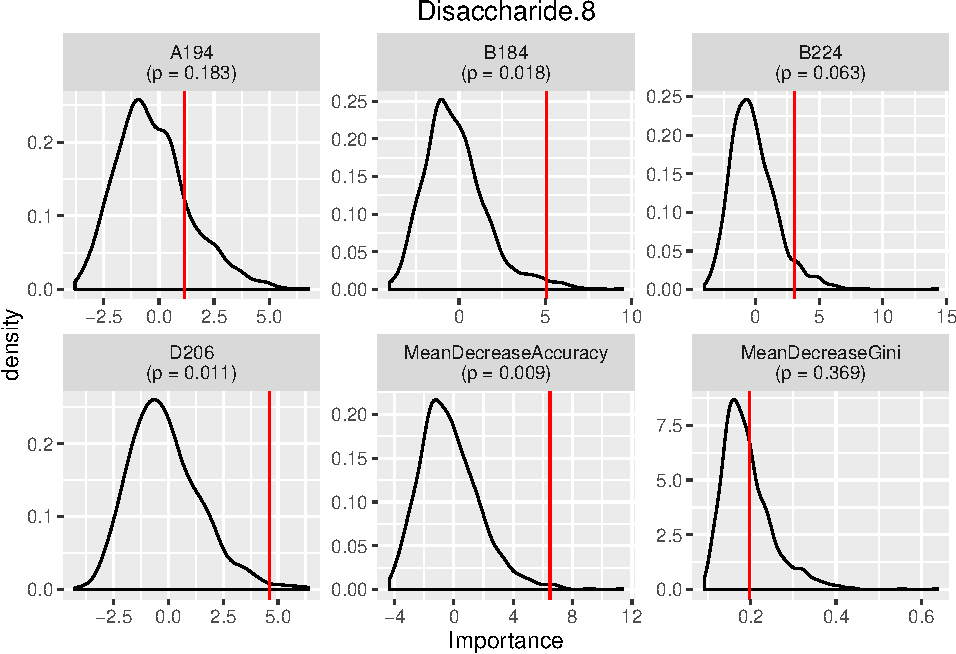
\includegraphics{archer_files/figure-latex/plotNull-1} \end{Schunk}

An ordered bar chart of all predictor importances with designations of
their significance at a specified critical alpha (traditionally 0.05),
can be visualized with the \texttt{plot} function applied to the result
of \texttt{rp.importance}. Here we show the distribution of importance
values for all predictor metabolites for Mean Decrease in Accuracy. Bars
that are colored red have p-values \textless{}= 0.05:

\begin{Schunk}
\begin{Sinput}
plot(imp, type = "MeanDecreaseAccuracy")
\end{Sinput}

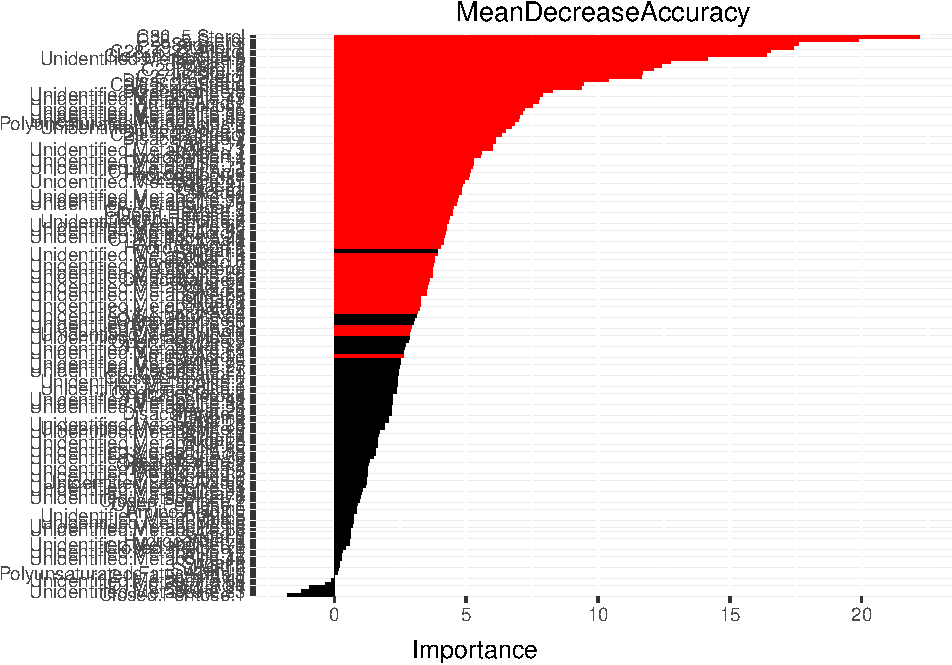
\includegraphics{archer_files/figure-latex/plot_imp1-1} \end{Schunk}

This shows that approximately the top third of the predictor metabolites
are deemed significant at p \textless{}= 0.05, even though the
distributon of importance scores shows a steady decline with no obvious
break in this region. Given that we can't see much detail about specific
predictor metabolites, we can also show just the top 10 most important
predictors, but this time for all importance types:

\begin{Schunk}
\begin{Sinput}
plot(imp, n = 10)
\end{Sinput}

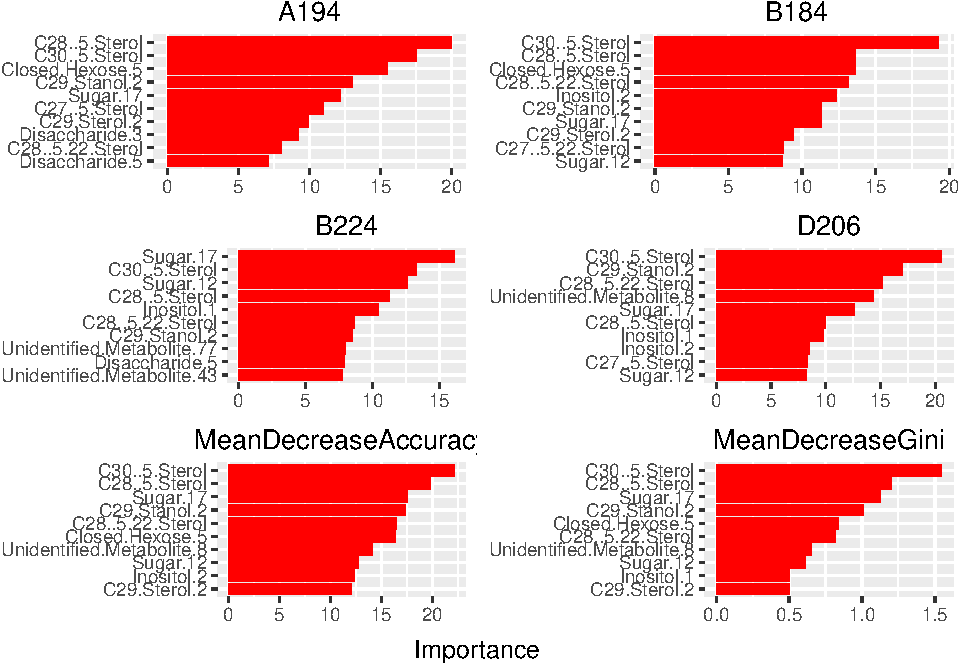
\includegraphics{archer_files/figure-latex/plot_imp2-1} \end{Schunk}

This shows that many of the same metabolites are significantly important
for all classes. To better visualize the relative distribution of
predictor importance across classes we can also produce a heatmap, with
cells shaded either according to the absolute value of importance, or by
rank. Here we display the top 50 most important predictors for each
class, color-coded by rank with significant predictors outlined in
black:

\begin{Schunk}
\begin{Sinput}
impHeatmap(metab.rf, n = 30)
\end{Sinput}

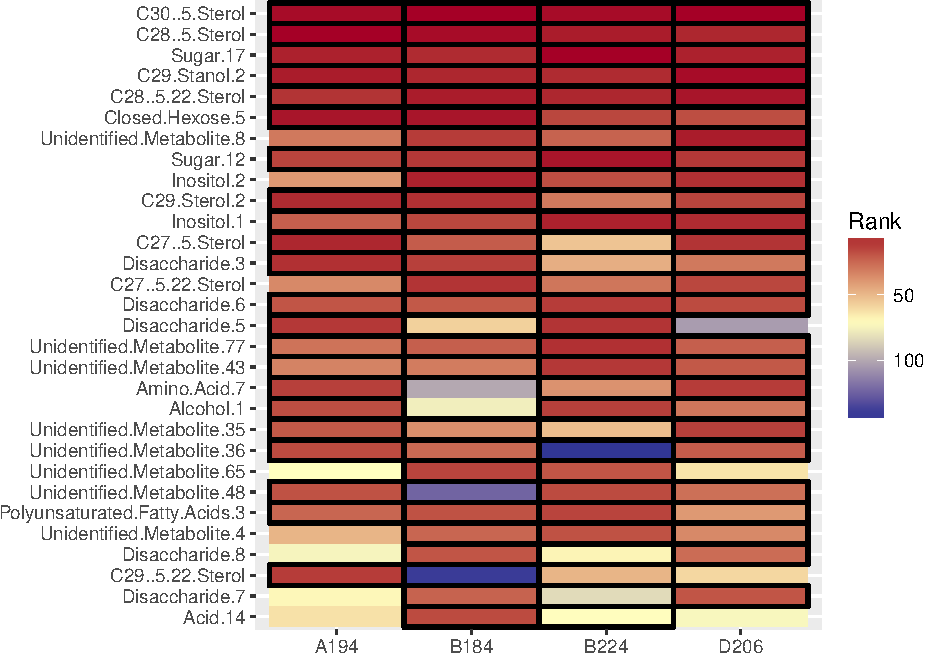
\includegraphics{archer_files/figure-latex/impHeatmap-1} \end{Schunk}

Although many of the same metabolites rank high for all classes, there
are several lower down in the list that are significant in some classes,
but not in others, suggesting that they have strong diagnostic
properties for those subsets of classes.

\subsection{Model summary functions}\label{model-summary-functions}

\texttt{rfPermute} also provides a set of convenient summary functions
for \emph{randomForest} models, regardless of predictor significance was
estimated by \emph{rfPermute} or not. For classification models, in
order to evaluate how well the model is performing, one should compare
the observed OOB error rates to what would be expected if samples were
just randomly allocated to bins in the absence of information from
predictor variables. This rate turns out to simply be the fraction of
the total sample size represented by each class. In a simple two-class
model, with equal sample sizes in each class, this is then 50\% for both
classes. However, if the sample sizes are skewed, say 80 in class A, and
10 in class B, then one would expect on average to correctly classify 80
/ 90 of the class A samples and 10 / 90 of the class B samples. Thus the
expected error rates would be 0.11 for class A and 0.89 for class B.
These values, referred to as ``priors'' are calculated by the
\texttt{exptdErrRate} function. Since this data set has equal sample
sizes, all priors are the same:

\begin{Schunk}
\begin{Sinput}
exptdErrRate(metab.rf)
\end{Sinput}
\begin{Soutput}
#>  OOB A194 B184 B224 D206 
#> 0.75 0.75 0.75 0.75 0.75
\end{Soutput}
\end{Schunk}

The \texttt{classConfInt} function provides confidence intervals for the
class-specific and overall model classification scores based on a
binomial distribution. This helps provide a measure of uncertainty of
the true classification rate given the observed sample sizes:

\begin{Schunk}
\begin{Sinput}
classConfInt(metab.rf)
\end{Sinput}
\begin{Soutput}
#>         pct.correct  LCI_0.95  UCI_0.95 Pr.gt_0.8
#> A194       0.875000 0.6165238 0.9844864 0.8592625
#> B184       0.937500 0.6976793 0.9984189 0.9718525
#> B224       0.937500 0.6976793 0.9984189 0.9718525
#> D206       0.937500 0.6976793 0.9984189 0.9718525
#> Overall    0.921875 0.8270217 0.9741462 0.9979437
\end{Soutput}
\end{Schunk}

A complete summary of the \emph{randomForest} classification model can
be produced by combining the results of \texttt{classConfInt} and
\texttt{exptdErrRate} along with the full confusion matrix as in the
function, \texttt{confusionMatrix}:

\begin{Schunk}
\begin{Sinput}
confusionMatrix(metab.rf)
\end{Sinput}
\begin{Soutput}
#>         A194 B184 B224 D206 pct.correct LCI_0.95 UCI_0.95 Pr.gt_0.8 Prior
#> A194      14    1    1    0     87.5000 61.65238 98.44864  85.92625    25
#> B184       0   15    0    1     93.7500 69.76793 99.84189  97.18525    25
#> B224       0    0   15    1     93.7500 69.76793 99.84189  97.18525    25
#> D206       0    1    0   15     93.7500 69.76793 99.84189  97.18525    25
#> Overall   NA   NA   NA   NA     92.1875 82.70217 97.41462  99.79437    25
\end{Soutput}
\end{Schunk}

Note that in this matrix, the \texttt{pct.correct} column is 100 * (1 -
OOB error rate) as I have found that this scale is more readily
comprehended by people unfamiliar with Random Forest or classification
algorithms.

\subsection{Vote distributions}\label{vote-distributions}

When evaluating a Random Forest model, it can be useful to visualize the
distribution of votes for classes within the forest. From these
distributions, we can tell if individual cases are tending to be
correctly classified with large probabilities (have a high fraction of
trees voting for the correct class), or have equivocal assignments (vote
probabilities are roughly equal). We can also see if misclassified
samples were strongly or weakly misclassified. The \texttt{plotVotes}
function will produce such a distribution, either as a bar chart, which
is useful when few samples are present, or as an area chart, which is
more readable with many samples:

\begin{Schunk}
\begin{Sinput}
plotVotes(metab.rf)
\end{Sinput}

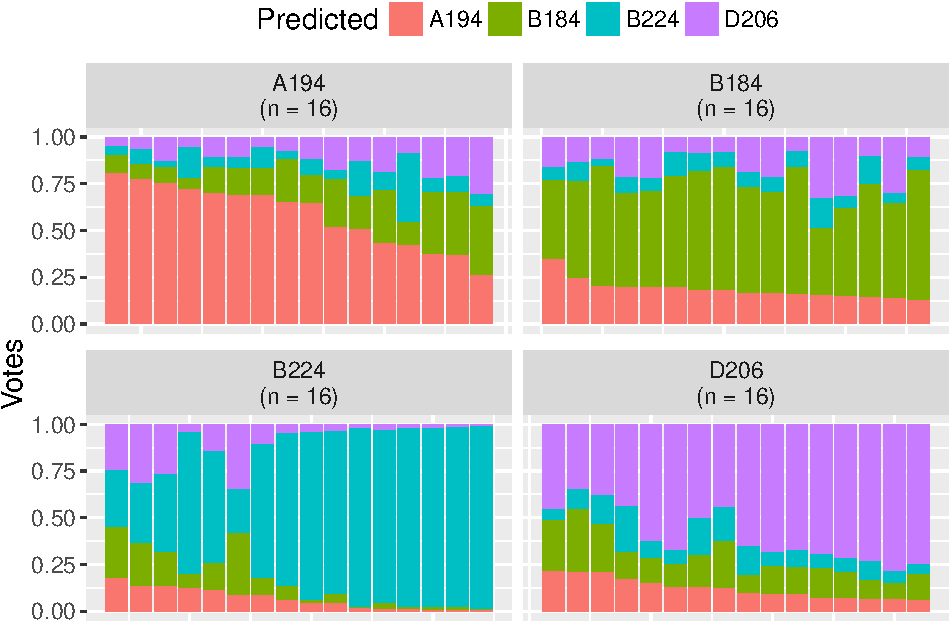
\includegraphics{archer_files/figure-latex/plotVotes-1} \end{Schunk}

Here we can see that \emph{Symbiodinium} types A194 and D206 have many
of their members classified with a relatively large fraction of votes.
We also see that the two B224 samples that were misclassified to D206
only had about 30\% of the votes to D206, which is not a strong
misclassification.

\subsection{Proximity plots}\label{proximity-plots}

For visualizing the relative distribution of samples in the Random
Forest, multi-dimensional scaling (MDS) is applied to the proxmity
matrix computed by \texttt{randomForest}. The \emph{randomForest}
package provides the \texttt{MDSplot} function which uses base graphics
to visualize these points. In \emph{rfPermute} there is the
\texttt{proximityPlot} function which uses \emph{ggplot} graphics and
provides a few additional useful features. The result of
\texttt{proximityPlot} depicts the MDS project of cases, with classes
encircled by a shaded convex hull. Additionally, each case is
represented by a color-coded dot and circle. The color of the interior
dot corresponds to the original case, while the color of the exterior
circle corresponds to the predicted case. Thus, correctly classified
cases will have the same color, while misclassified cases will have
different colors, as in this example:

\begin{Schunk}
\begin{Sinput}
proximityPlot(metab.rf)
\end{Sinput}

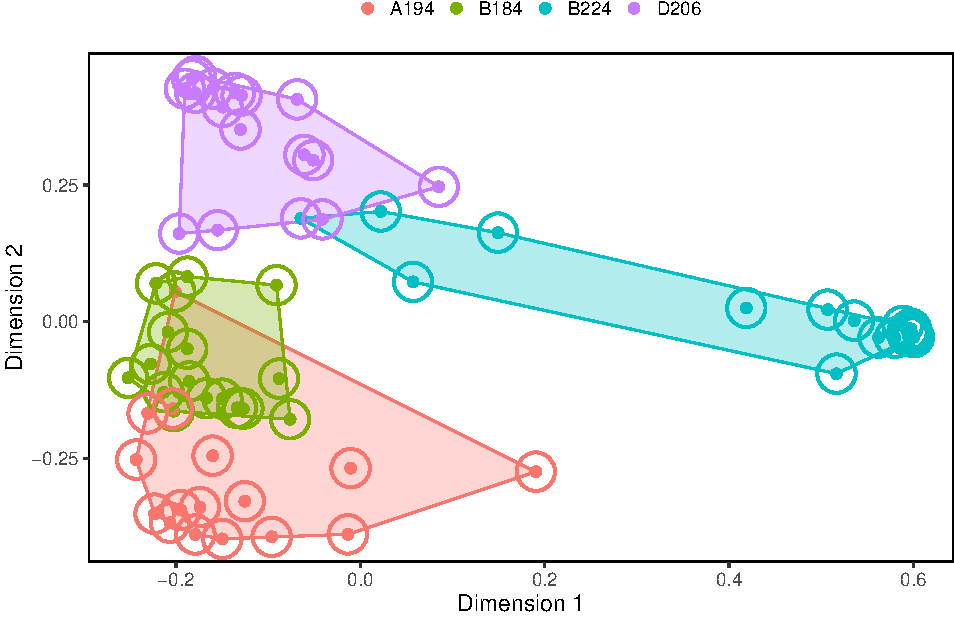
\includegraphics{archer_files/figure-latex/proximityPlot-1} \end{Schunk}

Here we can see the two misclassified B224 samples on the periphery of
the D206 convex hull, some distance away from the majority of the other
B224 samples, but also separated from the majority of the D206 samples.
Given the variability in B224, we might then view these as aberrant B224
samples rather than mislabelled D206 samples.

\subsection{Performance}\label{performance}

Because the primary function, \texttt{rfPermute}, is a wrapper that
calls \texttt{randomForest} multiple times, execution time can be
lengthy for large data sets and will scale relatively linearly with the
number of permutations. However, execution time can be reduced if a
multi-core machine is used and the \texttt{num.cores} argument set
appropriately. For example, on a MacBook Pro with a 2.8GHz Intel Core i7
chip and 16GB of 1600 MHz DDR3 RAM, one \texttt{randomForest} run of the
\emph{Symbiodinium} data set took approximately 0.1 seconds. The same
\texttt{rfPermute} model with 100 replicates took 14.4 seconds, and 1000
replicates took 142.3 seconds. When the number of cores used was
increased from one to three, the 1000 replicate model took 46 seconds.

\subsection{Installation}\label{installation}

The stable version of \emph{rfPermute} can be installed from CRAN via:

\begin{Schunk}
\begin{Sinput}
install.packages('rfPermute')
\end{Sinput}
\end{Schunk}

To install the latest development version from GitHub, use:

\begin{Schunk}
\begin{Sinput}
# make sure you have Rtools installed
if (!require('devtools')) install.packages('devtools')

# install from GitHub
devtools::install_github('EricArcher/rfPermute')
\end{Sinput}
\end{Schunk}

\bibliography{RJreferences}

\address{%
Frederick I. Archer\\
Southwest Fisheries Science Center\\
8901 La Jolla Shores Drive\\ La Jolla, CA 92037 USA\\
}
\href{mailto:eric.archer@noaa.gov}{\nolinkurl{eric.archer@noaa.gov}}

